\begin{chapter}{Decision Analysis \label{Ch:decision}}
\section{Introduction}
A large number of factors are present in the development of an offshore windfarm. Consider a finite number of hypothetical windfarms that could be built, but we are only able to build one such windfarm. Which do we choose? Suppose for now we are the only stakeholder. More realistically there could be investment from government as well as private investors. How do we come to the decision of which windfarm is the best? Ultimately, we need to hypothesise what the consequences of building each possible windfarm might be. We then need to evaluate how good (or bad!) such consequences are as well as how likely any set of possible consequences are. A mathematical framing of this task is to set it up as a decision problem; the decision which maximises our expected utility is the `best' decision to make from any decision $d$ in the space of all possible decisions $\mathcal{D}$.

Using a Bayesian decision analysis framework, the optimal decision, $d^\star$ is the decision which maximises the expected utility of the decision. That is,

\begin{equation}
d^\star = \argmax_{d \in \mathcal{D}} \E_{\mathcal{P}_d} \{u(d)\}. \label{Eq:optimal-decision}
\end{equation}

This expectation depends on two things
\begin{enumerate}
	\item[(i)] $\mathcal{P}_d$ --- the probability distribution over the consequences of a decision if that decision were to be made.
	\item[(ii)] $u(\cdot)$ --- the utility function. The utility function returns a value corresponding how desire able a consequence is; a higher value indicates a more desirable consequence.
\end{enumerate}

In many problems, it is enough (and even encouraged) to use an ``off the shelf'' utility function. For instance, in Bayesian optimal design, the ``decision'' is choosing the design of the experiment (perhaps choosing the time at which measurements are taken to have the `best' experiment). An experiment might be performed to estimate model parameters hence a Bayesian optimal design might be chosen to maximise the amount learned about those parameters. A utility function might have good information theoretic properties in this scenario, so the decision maker (DM) might choose to maximise the Kullback Leibler (KL) divergence between the prior distribution and posterior distribution of parameters; a large KL divergence from prior to posterior suggests the data have been highly informative. A recent review of useful utility functions in Bayesian optimal design is given in \citet{Ryan2016}.

In many industry problems there are many competing objectives; not all are immediately obvious or well-defined. For example, the energy output of the windfarm will want to be maximised, the upfront as well as operation and maintenance costs will want to be minimised. The decision maker is aware that a small upfront cost might only be made possible by purchasing components with a short expected lifetime which would drive up the maintenance costs and reduce availability; they are conflicting. Beyond this, the location of the windfarm will be important, too far from the shore and it will be too difficult to repair; if it is too close to the shore there and it will be much less windy (therefore reduced scope for energy generation) as well as potential opposition from local residents; their beloved coastal views are ruined. Further, there are safety aspects to consider. A risky (but potentially profitable) windfarm might pose threat to the health and safety of the maintenance engineers. There will of course be other concerns, this is not an exhaustive list. Since problems such as the design of a windfarm are highly specialised, it might not be entirely surprising that an ``off the shelf'' utility function does not reflect what it most important in the problem. Further, what is important will not be consistent across possible decision makers or even at different times to the same decision maker. A bespoke utility function which reflects the DM's preferences over all possible consequences at the time of making the decision is an attractive approach. To construct such a function, the DM needs to specify many things, including the attributes (the measurements associated to consequences) as well as how important each attribute is as well as how preferable each possible consequence is. This is not a trivial task and each decision maker will have their own utility function for the same problem, possibly with different attributes. We therefore have to elicit the DM's utility function for the problem at hand.

There is also the task of eliciting the probability distribution over the consequences; each decision imposes its own probability distribution over the set of possible consequences. Standard elicitation techniques can be used to construct each distribution; for a review see \citet{Garthwaite05,Ohagan06}. The expectations in \Cref{Eq:optimal-decision} are taken over these elicited (prior) probability distributions, $\mathcal{P}_d$. If relevant data is available at the time of making the decision, the expectation could be taken with respect to the posterior probability distributions, $\mathcal{P}_d | \bx$. Large portions of this chapter are based upon \citep{Keeney1976,Smith2010,ElicitationBook}, with references to particular chapters of \citet{ElicitationBook} and other materials where appropriate.

\section{Bayesian Networks \label{Sec:BNs} }

When the DM's beliefs sit in a high dimensional space, structuring the attributes of utility functions, and probability distributions over these beliefs is not straight forward. Bayesian Networks (BNs) are a useful, graphical tool to structure such quantities.

\subsection{Relevance}

If a vector measurement $\bX$ is of no ``relevance'' in predicting another vector $\bY$ then it is sensible to say $\bX \indep \bY$. Note that this does not require the DM to commit to any quantitative statement; it is a qualitative one (a very useful one at that!). Hence if our utility function is a function of $\bY$ (which is probabilistically independent of $\bX$), this independence simplifies the specification; we need only to think about $\bY$. This is also a time saving device (and possibly of financial benefit); specifying probability distributions is time consuming.

This simple form of independence is perhaps too simple for many practical problems of interest. Now let $(\bX, \bY, \bZ)$ be attributes defining the DM's problem. If the client believes that $\bX$ is irrelevant in predicting $\bY$ once $\bZ$ has been learned, (written $\bY \indep \bX | \bZ$).

Then, if the DM is a Bayesian, they will be able to express their joint density over $(\bX, \bY, \bZ)$ as

\begin{equation}
p(\bx, \by, \bz) = p(\by | \bz) p(\bx | \bz) p(\bz)
\end{equation}

because their conditional independence implies $p(\by | \bx, \bz) = p(\by | \bz)$.

Note that, whilst two experts might strongly agree that, for example, the probability that an absurd tweet from philanthropist Elon Musk causes a crash in Tesla stock prices in the next $6$ months is completely independent of the probability that South Shields FC ever get the promotion to the National League North they truly deserve, the experts could have strongly disagreeing probability distributions over these measures.

Certain combinations of independence statements can lead to rather nice probability distributions. Here we provides a two examples:

\subsubsection*{Gaussian}

If $\bX_1 \indep \bX_2$ and $\bX_1 + \bX_2 \indep \bX_1 - \bX_2  $ then each $\bX_i \sim \mathcal{N}(\mu_i, \sigma^2)$ independently. Take note of the common variance.

\subsubsection*{Gamma-Beta}

If $\bX_1 \indep \bX_2$ and $\bX_1 + \bX_2 \indep \bY$ with $\bY = \frac{\bX_1}{\bX_1 + \bX_2}$ then this is equivalent to saying $\bX_i \sim Gamma(\alpha_i, \beta)$ (common $\beta$) and it is possible to show that $\bY \sim Beta(\alpha_1, \alpha_2)$.


\subsection{Bayesian Networks \& DAGs}

This section treats the cases in which the decision space is relatively simple (a manageable number of discrete decisions) but the complexity is due to the relationships between the variables being complex and large in number. The following section is heavily based on Chapter $7$ of \citet{Smith2010}.

A depiction of the DM's explanations of such relationships should have the following properties

\begin{itemize}

	\item Evocative and understandable; the DM has ownership.
	\item Provides a faithful picture of the pattern of relationships the DM believes exists between features of the problem.
	\item The topology links to a set of statements about (conditional) independence obeying semi-graphoid properties. The graph therefore has local integrity enabling logical consequences of the DM's statements to be fed back to her ensuring the faithfulness of the graphical representation.
	\item It is possible to embellish the graph with probability distributions provided by the DM. This embellishment should not void any of the previously elicited (conditional) irrelevance statements.
	\item This framework can be used as a guide to Bayesian learning \& fast computation.

\end{itemize}

The most used such depiction is the Bayesian Network (BN). The BN avoids at the early stages eliciting \textit{numerical} quantities allowing the DM to focus on the main features and patterns within her belief structure.

\subsection{The Bayes Net and Factorisiations}

One of the easiest ways to think of a BN is a factorisation. If we are expressing beliefs over $\bX = (x_1, \ldots, x_n)$ we can write:

\begin{equation}
	p(\bx) = p_1(x_1)p_2(x_2|x_1)p_3(x_3|x_1, x_2) \cdots p_n(x_n|x_1, x_2, \ldots, x_{n-1}). \label{Eq:cond-mass}
\end{equation}

Conditional independence statements allow us to simplify \Cref{Eq:cond-mass}, since if $\bY \indep \bZ | \bX$ then $p(\by | \bx, \bz) = p(\by | \bx)$ for any random vectors $\bX, \bY, \bZ$ and any density function $p(\cdot)$.

Now written in terms of a random vector $\bX = (X_1, \ldots, X_n)$, if we let $Q_i \subset \{1, \ldots, i-1\}, 2 \leq i \leq n $ where the \textit{parent} set is $Q_i \subseteq \{1, \ldots, i-1\}$ and the \textit{remainder} set is $R_i = \{1, \ldots, i-1\} \backslash  Q_i$ then $p(\bx)$ has the following factorisation:

\begin{equation}
	p(\bx) = p_1(x_1) \prod_{i=2}^n p_i(x_i | \bx_{Q_i}).
\end{equation}

This is equivalent to $X_i \indep \bX_{R_i} | \bX_{Q_i}$.

We now need a definition: A directed acyclic graph (DAG) is a graph $\mathcal{G} = (\mathcal{V}, \mathcal{E})$ where $\mathcal{V}$ is the set of vertices connected by edges $\mathcal{E}$; the graph is a directed graph having no directed cycles.

We  are now in the position to define a Bayesian Network:
A Bayesian Network (BN) on $\bX = \{X_1, \ldots, X_n\}$ is the set of $(n-1)$ conditional independence statements together with a DAG $\mathcal{G} = (\mathcal{V}, \mathcal{E})$. The set $\mathcal{V}$ of vertices is $\{X_1, \ldots, X_n\}$; a directed edges from $X_i$ to $X_j$ is in $\mathcal{E}$ if and only if $i \in Q_j$, $1\leq i$, $j \leq n$. The DAG is valid if the DM believes the conditional independence statements associated with the BN.

Here we present an example. If the DM has a problem defined by $5$ measurements $(U, V, X, Y, Z)$ and she believes that $p_2(v|u)$ depends on $u$, $v$; $p_3(x|u,v)$ depends on $x$, $v$; $p_4(y|u,v,x,)$ depends on $x$, $v$; and $p_5(z|u, v, x, y)$ depends on $x$, $z$. Her corresponding DAG is then given in \Cref{Fig:dag1}.

\begin{figure}
	\centering
	\begin{tikzpicture}[node distance = 2cm, auto]
		%place nodes = RVs
		\node [cloud] (U) {U};
		\node [cloud, right of = U] (V) {V};
		\node [cloud, right of = V] (X) {X};
		\node [cloud, below of = X] (Y) {Y};i
		\node [cloud, right of = X] (Z) {Z};
		% draw edges
		\path [line] (U) -- (V);
		\path [line] (V) --(X);
		\path [line] (V) -- (Y);
		\path [line] (X) -- (Y);
		\path [line] (X) -- (Z);
	\end{tikzpicture}
	\caption{An example of a DAG.}
	\label{Fig:dag1}
\end{figure}

\subsection{Eliciting the BN}

There exist off the shelf BNs, but they are typically suited to designed experiments that fit into a standard hierarchical structure. We will require more bespoke solutions. We now demonstrate a protocol for the elicitation of a BN with decision analysis in mind.

The BN elicitation has three main steps:

\begin{enumerate}
		\item Defining the variables.
		\item Clarifying the explanatory variables.
		\item Drawing the Bayesian Network.
\end{enumerate}

Clearly each step is complex. We will elaborate on each step in turn in the context of the DM being a senior employee at an energy firm who is considering the construction of an offshore windfarm. It is worth stressing that the DM is exploring the consequences following a particular fixed policy or decision rule.


\subsection{Defining the variables}

The initial random variables are the attributes of the DM's utility function --- Level $1$ quantities. The DM could simply assess the the profit implication of constructing am offshore windfarm. More realistically, the DM is also concerned with how the public respond to a large structure being built in the area and the health and safety of those constructing and maintaining the windfarm. This completes the Level $1$ quantities.

We now ask the DM to consider other features of the problem which might have a direct influence on at least one attribute; the Level $2$ features. For example, the profit depends on how much energy is generated as well as the energy demand and the cost of maintaining the windfarm. Another Level $2$ variable will be the distance from the shore that the windfarm is built; if it is far away it will have minimal visibility and potentially less opposition from local residents. A level $3$ feature might be the upfront cost of the windfarm; if a lot of money is spent on the design and construction of the windfarm using the best possible components, this could maximise energy generation. This ultimately depends on the design of the windfarm, so a level $4$ feature will be the windfarm design.

\tikzstyle{cloud} = [draw, ellipse, fill=red!20, node distance = 3cm, minimum height = 3em, text width = 2cm]
\begin{figure}

	\centering

	\begin{tikzpicture}[auto, align = center]
		%place nodes = RVs
		% \node [cloud] (name) {text};
		\node [cloud] (Profit) {Profit};
		\node [cloud, right = 1cm of Profit] (Fatalities) {Fatalities};
		\node [cloud, below = 0.5 cm of  Profit] (En-Gen) {Energy \\ Generated};
		\node [cloud, below = 0.5 cm of En-Gen] (Up-Cost) {Upfront Costs};
		\node [cloud, below = 0.5 cm of Up-Cost] (Comps) {Windfarm Design};
		\node [cloud, right = 1cm of Up-Cost] (Train) {Quality of Training};
		\node [cloud, right = 1cm of En-Gen] (Main-Cost) {Maintenance Costs};
		\node [cloud, left = 1cm of En-Gen] (Demand) {Demand};
		\node [cloud, right = 1 cm of Fatalities] (Public) {Public Reaction};
		\node [cloud, below = 0.5 of Public] (Dist) {Distance from Shore};
		% draw edges
		\path [line, ultra thick] (En-Gen) -- (Profit);
		\path [line, ultra thick] (Up-Cost) -- (En-Gen);	
		%\path [line, ultra thick] (Up-Cost) to[out=180,in=200] (Profit);
		%\path [line, ultra thick] (Train) -- (En-Gen);
		\path [line, ultra thick] (Main-Cost) -- (Profit);
		\path [line, ultra thick] (Train) to[out=0,in=-20] (Fatalities);	
		%\path [line, ultra thick] (Train) -- (Main-Cost);
		%\path [line, ultra thick] (Comps) -- (Train);
		\path [line, ultra thick] (Comps) -- (Up-Cost);
		\path [line, ultra thick] (Demand) to[out=60,in=190] (Profit);
		\path [line, ultra thick] (Dist) -- (Public);
	\end{tikzpicture}

	\caption{The DM's trace-back graph.}

	\label{Fig:traceback}
\end{figure}

\subsection{Clarifying the Explanatory Variables}

The next stage of the elicitation is to categorise the features. We sort them into two sets: the ``explicit'' features which have a clear, unambiguous definition; remaining features are ``implicit'' since they do not yet have a measurable definition. A set of $5$ sufficient properties for an attribute is given by \citet{Keeney2005} as follows

\begin{enumerate}
\item[(i)] \textit{Unambiguous}: There is a clear relationship between consequences and their descriptions using the attribute.
\item[(ii)] \textit{Comprehensive}: For each objective, the corresponding attribute levels cover the range of possible consequences. Value judgements implied by that attribute are sensible.
\item[(iii)] \textit{Operational}: It is practically possible to obtain information to describe consequences; value trade-offs can reasonably be made.
\item[(iv)] \textit{Direct}: The attribute levels directly describe the consequences of interest.
\item[(v)] \textit{Understandable}: It is easy to understand and communicate clearly the consequences and value trade-offs made using the attribute.
\end{enumerate}

Even features with a currently unknown value can be explicit so long as their value can \textit{eventually} be learned. For example, the upfront cost of constructing the windfarm is currently unknown but can be measured unambiguously at some point after the work has been completed. Conversely, ``public reaction'' is not an explicit feature as it stands (nor is ``Quality of Training''); we need to specify precisely how this will be measured. (c.f. an observable quantity in eliciting probabilities \citep{Ohagan06}).

Explicit features can be treated as if they were an uncertain measurement; their lack of ambiguity allows them to be treated like an random variable. The next task is addressing the implicit features. We need to somehow transform these into explicit features. For example, consider the water company's public acceptability. In re-expressing the implicit features as explicit ones, it is common to uncover previously unspecified aspects of the problem.

If we cannot replace all the implicit features with explicit ones we should record all the remaining implicit features. We can then, instead of including these in the BN, refer back to them indirectly when judgements require input.

This subsection allows us to construct a ``trace-back'' graph which is \textit{not} a BN; an example is given in \Cref{Fig:traceback}. It does however specify the explicit features and a partial ordering of them given by their levels.

\subsection{Drawing the BN}

Here we aim to draw the (provisional) BN. The vertices given are the explicit features which shall be ordered by their levels. The higher the index; the lower the level the feature belongs to. We start with the trace-back graph as nodes; we draw in new nodes to encode the (conditional) independence where appropriate. A lack of edge between two nodes expresses they have some kind of irrelevance.

In the water company's context, label the features as follows:

\begin{itemize}

	\item{ $X_1 =$ Windfarm Design; expected lifetime of critical turbine components}
	\item{ $X_2 =$ Distance from the shore in miles}
	\item{ $X_3 =$ Upfront costs of windfarm construction in millions of pounds}
	\item{ $X_4 =$ Budget for health and safety and training in thousands on pounds}
	\item{ $X_5 =$ Annual energy demand from local town in Mega Watt hours}
	\item{ $X_6 =$ Annual energy generation of the windfarm in Mega Watt hours}
	\item{ $X_7 =$ Cost of maintaining the windfarm during its operational life in millions of pounds}
	\item{ $X_8 =$ Annual profit from the windfarm in millions of pounds}
	\item{ $X_9 =$ Number of fatal accidents as a result of construction and maintenance of the windfarm}
	\item{ $X_{10} =$ Number of negative articles about the windfarm published in newspapers during construction and operational life of the windfarm}

\end{itemize}

Any listing that is consistent with the reversed levels is allowed. If $X_9$ and $X_{10}$ were permuted then this would be fine --- they are both members of Level $1$. No features have been omitted here, but if for instance, the DM could not specify what would measure ``public reaction'' then it should have been dropped. However the DM decided that this could be measured by the number of negative press articles published about the windfarm, so was retained via this proxy variable.

Now starting second listed feature, we ask the DM which subset, $Q_i$, of indices are useful in prediction of $X_i$, $2 \leq i \leq n$. At one extreme, any $Q_i$ could be an empty set; knowing the values of the measurements prior to $X_i$ in the list is useless (and possibly a hindrance) in predicting $X_i$. At the other extreme, every variable listed prior to $X_i$ could be useful in predicting $X_i$.

In the windfarm example, we ask the DM whether the the expected lifetimes of components is related to the amount of money spent on health and safety training. The DM reports that she cannot see any possible link between the two variables, hence no edge will be placed between $X_1$ and $X_4$. The DM is then asked if either of $X_1$ or $X_2$ would be useful in predicting $X_3$; the answer is that just $X_1$ is a useful predictor, so no new edges are drawn. In asking what would be useful in predicting $X_6$, the DM says the distance from shore is a useful predictor --- the wind is stronger far away from the coast and hence more energy could be produced, so an edge from $X_2$ to $X_6$ is drawn.

The process continues to question the DM until we have considered what variables might predict $X_n = X_{10}$. The DAG can then be drawn; see \Cref{Fig:provis-BN}.
\tikzstyle{cloud} = [draw, ellipse, fill=red!20, node distance = 3cm]
\begin{figure}[H]
	\centering
	\begin{tikzpicture}
		%% nodes

		%level 1

		\node [cloud] (Profit) {$X_8$};
		\node [cloud, right = 1cm of Profit] (Fatalities) {$X_9$};
		\node [cloud, below = 0.5 cm of  Profit] (En-Gen) {$X_6$};
		\node [cloud, below = 0.5 cm of En-Gen] (Up-Cost) {$X_3$};
		\node [cloud, below = 0.5 cm of Up-Cost] (Comps) {$X_1$};
		\node [cloud, right = 1cm of Up-Cost] (Train) {$X_4$};
		\node [cloud, right = 1cm of En-Gen] (Main-Cost) {$X_7$};
		\node [cloud, left = 1cm of En-Gen] (Demand) {$X_5$};
		\node [cloud, right = 1 cm of Fatalities] (Public) {$X_{10}$};
		\node [cloud, below = 0.5 of Train] (Dist) {$X_2$};
		% draw edges
		\path [line, ultra thick] (En-Gen) -- (Profit);
		\path [line, ultra thick] (Up-Cost) -- (En-Gen);	
		%\path [line, ultra thick] (Up-Cost) to[out=180,in=200] (Profit);
		%\path [line, ultra thick] (Train) -- (En-Gen);
		\path [line, ultra thick] (Main-Cost) -- (Profit);
		\path [line, ultra thick] (Train) to[out=0,in=-20] (Fatalities);	
		\path [line, ultra thick] (Train) -- (Main-Cost);
		%\path [line, ultra thick] (Comps) -- (Train);
		\path [line, ultra thick] (Comps) -- (Up-Cost);
		\path [line, ultra thick] (Demand) to[out=60,in=190] (Profit);
		\path [line, ultra thick] (Dist) to[out=0,in=-90] (Public);
		\path [line, ultra thick] (Dist) to[out=180,in=-30] (En-Gen);
		\path [line, ultra thick] (Dist) to[out=20,in=-5] (Fatalities);
		\path [line, ultra thick] (Dist) to[out=150,in=200] (Main-Cost);

	\end{tikzpicture}
	\caption{The DM's BN for the water renovation example.}
	\label{Fig:provis-BN}
\end{figure}

The BN construction allows us to simplify the elicitation. If the value of an explicit feature can be known with certainty at the time of the decision then no further information is require to forecast it. Therefore, this vertex need have no parents; it is a root vertex. If such features can be identified then then we do not have to dig into the predictors of this feature.

We also stress here that the trace-back graph is not a BN. The trace-back graph tells us which features \textit{should} be related by including an edge in the diagram. However, the BN denies the possibility of a relationship between two variables by the absence of an edge between their nodes.

The BN can be further refined; the DM might believe that more edges should be added. The DM is  comfortable that the BN represents her beliefs about how all the relevant features of the problem are connected to one another. The BN does not express everything the DM believes and wants to express. For example, we do not yet have a distribution over $\bX$; but a skeleton of it. We must now carefully elicit this probability distribution; the BN provides a good starting point.

\section{A Procedure For Eliciting Utility Functions}

It is common to use off-the-shelf utility functions for well defined problems. However, many real world problems are not well defined thus require a bespoke, subjective utility function. This utility function belongs to the DM and must be elicited in some way. In \Cref{Sec:BNs} we discussed how to obtain attributes of the utility function. We must now find a way to assign a utility to all possible combinations of the attributes; we need to specify the DM's own utility function for the problem at hand. This section is based upon \citet{Gonzalez2018}.

To elicit the DM's utility function over more than one attribute, we need to first elicit the individual utility functions over each attribute. Hence we will first cover some of the basics of utility theory and univariate utility elicitation.

\subsection{Fundamental Utility Notions}

There are three axioms of utility theory under risk where a preference relation $\preceq$ is assumed on a probability space $\mathcal{P}$. The axioms are as follows:

\begin{enumerate}
	\item \textbf{Weak-order:} $\preceq$ on $\mathcal{P}$ is complete; $\forall$ $p, q \in \mathcal{P}$ either $p \preceq q$ or $q \preceq p$ and is transitive; $\forall p, q, r \in \mathcal{P}$  $p \preceq q$ together with $q \preceq r$ $\implies$ $p \preceq r$.

\item \textbf{Archimedian:} $\forall p, q, r \in \mathcal{P}$ if $p \prec q \prec r$ then $\exists \alpha, \beta \in (0, 1) $ such that $\alpha p + (1-\alpha)r \prec q \prec \beta p + (1-\beta) r$
\item \textbf{Independence:} $\forall p, q, r \in \mathcal{P}$ and $\alpha \in (0, 1]$, $\alpha p + (1-\alpha)r \preceq \alpha q + (1-\alpha r) \iff p \preceq q$.
\end{enumerate}

Under these conditions there is a \textit{utility function}, $u$, satisfying $\forall p, q \in \mathcal{P}$

\begin{enumerate}
\item[(i)] $p \preceq q \iff u(p) \leq u(q)$
\item[(ii)] $u(\alpha p + (1-\alpha) q) = \alpha u(p) + (1- \alpha)u(q)$
\end{enumerate}

from this it is straightforward to deduce $p \preceq q \iff \E_p(u) \leq \E_q(u)$.

Note that a utility function is only unique up to a positive affine transformation; $a^2u(\cdot) + b$ for $a, b, \in \mathbb{R}$ represents the same set of preferences as $u(\cdot)$.

\section{A Single Attribute Elicitation Protocol}

Let the consequence space be $\mathcal{C}$; this is the ``input'' space for the utility function. The simplest case has two fixed consequences $x^0 \prec x^*$; for each $x \in \mathcal{C}$ with $x^0 \preceq x \preceq x^*$ the DM will specify a value $p \in [0, 1]$ for which she is indifferent between two gambles; gamble A is to obtain $x$ for certain, gamble B is to obtain $x^* U + (1-U)x^0$ where $U \sim Bernoulli(p)$. Gamble B can be concisely expressed as $[x^*, x^0 ; p]$.

If the DM is indifferent between gambles A and B then $x$ is the \textit{certainty equivalent} for $[x^*, x^0; p]$. They are equally preferable, $\text{A} \sim \text{B}$, therefore they must have equal expected utility:

\begin{align}
	u(x) & = pu(x^*) + (1-p)u(x^0)\\
	     & = p \times 1 + (1-p) \times 0 \\
	     & = p.
\end{align}

This holds because we have assumed, and can do so without loss of generality (due to utility functions being unique up to positive affine transformations), that $u(x^*) = 1$ and $u(x^0) = 0$.

Hence, a fairly primal elicitation procedure is as follows:

\begin{enumerate}
	\item Determine $[x^0, x^*]$; the range for the attribute of interest.
	\item Set $u(x^*) = 1 - u(x^0) = 1$.
	\item Assign utilities $\{u_1, \ldots, u_n\}$ to a set of intermediate values $\{x_1, \ldots, x_n\}$.
	\item Fit a utility function to the data $\{(x^0, 0), (x_1, u_1), \ldots, (x_n, u_n), (x^*, 1) \}$. This can be done via a least squares procedure.
	\item Check for consistency; ask a few verification questions.
\end{enumerate}

Note that the above recipe assumes a given functional form for $u(\cdot)$; choosing this functional form can be tricky. Further, assigning utility values to intermediate values is not trivial. The utilities can be assigned imprecisely or precisely and it is also important to be aware of, and counter, the DM's inaccuracies and biases.

The main point of the above produce is point $3$: assigning utilities. The number $n$ of utilities to be assigned will be a trade off between accuracy of the resulting utility function and the time available.

There are two main ways to elicit utilities. The first is \textit{probability equivalence}: the DM is asked to specify $p$ such that $[x^*, x^0; p] \sim x$ for some predetermined, deterministic consequence, $c$. The second is \text{certainty equivalence}: the DM must specify $x$ such that $[x^*, x^0; p] \sim x$ for a predetermined $p$. If the DM and analyst agree to be precise, this can be achieved by specifying a range for the given quantity. For example, a certainty equivalent can be made imprecise by the DM stating that $(x', x'')$ is indifferent to  $[x^*, x^0; p]$. This then gives us a permissible region in which the DM's ``true'' $u(\cdot)$ will lie. Imprecision can also be employed when there are multiple decision makers who cannot agree on a certainty equivalent \citep{Farrow2009, Farrow2010}. Similarly, an interval for $p$, $(p' ,p'')$ could be specified by the DM to compare $[x^*, x^0; p]$ to a given certain consequence, $x$. 

\subsection*{Probability Equivalence}

Here the DM specifies their utility function by reporting probabilities. We review three methods for doing so.

\subsubsection*{Extreme Gambles}

We consider gambles and certainties of the form $[x_l, x_u; p_i]\sim x_i$. The reference points in this case are the extremes of $\mathcal{C}$. This is a straightforward procedure, but prone to bias from range effects, especially if the limits are too extreme.

\subsubsection*{Adjacent Gambles}

$[x_{i-1}, x_{i+1}; p_i] \sim x_i$. Similar to above but instead of using the extremes as reference points, we use ``locally best and worst'' scenarios for each $x_i$.


\subsubsection*{Assorted Gambles}

$[x_{j_i}, x_{x_i}; p_i] \sim x_i$. With $j_i < i < k_i$. This is a generalisation of adjacent gambles, allowing more freedom in the reference consequences.

\subsection*{Certainty Equivalence}

Here the DM specifies their utility function by reporting probabilities. We review three methods for doing so.

\subsubsection*{Fractile}

This is the analogue of extreme gambles; specify $x_i$ such that $[x^0, x^*;p_i]\sim x_i$. Biases can be present from range effects, there can also be distortions in risk behaviour when $p_i$ is too close to $0$ or $1$.

\subsubsection*{Chaining}

$[x_{i'}, x_{i''}; p_i] \sim x_i$. Here, $x_{i'}, x_{i''} \in S_{i-1} = S_{i-2}\cup x_{i-1}$ where $S_0  =\{x^0, x^*\}$. This allows us to assess utilities one at a time until enough points are available to estimate $u(\cdot)$ satisfactorily. Drawbacks include serial dependence, range effects and certainty effects.



\subsection{Risk Attitudes and Utility Functional Forms}

One of the most important issues is choosing the \textit{functional form} of the utility function. Two important features are: monotonicity (more profit is almost always preferred); concavity (a special reflection on the DM's behaviour).

Suppose $C \subset \mathbb{R}$ is the monetary consequence. For a lottery $p$ there are two expectations to consider. The \textit{expected utility} $\E_p[u(c)]$ and the expected (monetary) value $\E_{p} (x)$. The certainty equivalent is the amount of money the DM would place on a single play of the lottery; $u(x_p) = \E_p(u(x))$. Equivalently, $x_p = u^{-1} \left\{ \E_{p} (u(x)) \right\}$.

The risk premium is defined to be the difference between the expected value of the lottery, and its certainty equivalent. We can interpret this as the difference in the value of infinite plays of the lottery versus a single play:

\begin{equation}
	\pi_p = \E_p (x) - x_p.
\end{equation}

The sign of $\pi_p$ is a result of the shape of $u$. $u$ concave $\iff$ $\pi_p > 0$. Hence a risk averse decision maker prefers repeated playing of the lottery to a single play. In this scenario we call the DM \textit{risk averse}. A risk averse DM prefers a small deterministic payoff to a random payoff with larger expected value, but some chance of being very small, common in financial situations. A risk prone DM will prefer the lottery to it's expected consequence; a desperate individual may wish to spend their last $\pounds 1$ on a scratch card, the prospect of winning thousands is much more appealing than the fact that they will probably lose their stake and go hungry.

Of course, a decision maker does not have to be strictly risk prone or strictly risk averse. They could be risk neutral (in this case $u(x) = ax + b$) or they could have a varying attitude towards risk. For instance, suppose the DM is a student who is planning their revision strategy for a pass/fail exam. Suppose the pass mark is $60\%$. When considering their revision strategy, the DM is willing to do anything that will get them above the pass mark. However, the DM is not particularly bothered about achieving very high marks (although a very high mark would bring a level of personal achievement, which does increase the DM's utility of such events). For events below the pass mark, the DM will be risk prone, for events above the pass mark the DM will be risk averse; this leads to a sigmoidal shape. This is an example of the \textit{local} risk behaviour changing.

\subsection{Case Study: Utility Elicitation}

In this subsection we outline an example given by \citet{Gonzalez2018}. Serbia has had to spend large amounts of money to mitigate the impacts of natural disasters in their energy sector due to lack of prevention. A key objective is the minimisation of natural risks measured via the total amount spent on repairs of the energy infrastructure.

The best value for this criterion is $0$M\euro, no spending required. The worst value is $500$M\euro. We will proceed with a ``direct'' probability equivalence method.

Now the assessed utility of a cost $250$M\euro\ is $u(250) = 0.67$; that is the DM is indifferent between of a cost of $250M$\euro\ for sure or the lottery $500 X$M\euro\ where $X \sim Bernoulli(1 - 0.67)$. To arrive at this value, the DM is first offered $250$M\euro\ for sure or the option of $50/50$ lottery between $0$\euro\ and $500$M\euro. Since the DM preferred the certain amount, this suggests $u(250)>0.5$. So a new lottery was proposed where the probability of $0$M\euro\ was now $0.75$ hence $500$M\euro\ occurs with probability $0.25$. In this case the DM preferred the lottery so $u(250)<0.75$. This bisection procedure is iterated (6 iterations in this case) until the DM said they were indifferent between the certain loss $250$M\euro\ and the random loss $500 X$ with $X \sim Bernoulli (1-0.67)$. This procedure it then repeated for two other certain values; $100$M\euro\ and $400$M\euro. The utility function is this case is monotonically decreasing. The functional form $u(c) = 1 + \lambda(1 - \exp (\rho c))$ seems sensible. Fitting this functional form to the data via least squares gives $\hat{\lambda} = 0.15319$ and $\hat{\rho} = 0.00398$ which is consistent with risk averse behaviour. On a personal note, I probably would have reordered the $c$ axis so that $\tilde{c} = -c$. Hence $u(-500) = 0$ and $u(0) = 1$. There are some fairly simple numerical problems to overcome here too. For instance, to force $\rho >0$ we might want to re-parameterise; set $\rho = \theta^2$. Also, we might want to shift the units to increase the numerical stability of the estimates.

This not the only procedure for eliciting a utility function, an alternative method is the midpoint method (a type of chaining method). A procedure for eliciting utility functions, as part of a multiattribute problem, is given by \citet{Smith2010}. We begin by asking the DM for the best and worst values, $x^*$ and $x^0$. We then aim elicit $x[p]$ such that $u(x[p])=p$ for various values of $p$. The first such value is $p=0.5$; we ask the DM to specify $x[0.5]$ such that $x[0.5] \sim [x^0, x^*;0.5]$. We then ask the DM for $x[0.25]$, it is straightforward to see $x[0.25] \sim [x^0, x[0.5] ; 0.5]$. Alternatively we could ask for $x[0.75] \sim [x[0.5], x^*;0.5]$. We can keep bisecting $[0,1]$ until enough $x[p]$ as necessary have been specified. Least squares (or an exact fit where appropriate) can then be used to fit a functional form to the DM's preferences.

\section{Multi-Attribute Utilities}

Suppose $\mathcal{C} = \mathcal{C}_1 \times \mathcal{C}_2 \times \cdots \times \mathcal{C}_q \subset \mathbb{R}^q$ with $x = (x_1, x_2, \ldots, x_q)$. Certain independence conditions allow us to construct $u(\cdot)$ in an additive form. Such a form allows great a great deal of simplification in the elicitation of a multi-attribute utility function; if such simplifications were not present the DM could find the specification near to impossible.

Consider two gambles; gamble A is to receive $x$ for certain (composed of ``intermediate'' values) whereas gamble B is to receive $x^*U + x^0(1-U)$ with $U \sim Bernoulli(p)$. In this situation, the DM is being asked to simultaneously consider the trade-off between all $q$ attributes whilst taking into account her risk attitude. This is a congitively complex task; the DM is trying to consider many attributes simultaneously. Exploiting independence properties of utility and probability allows us to greatly simplify this procedure by considering attributes one at a time.

Now suppose $I \subset \{1, \ldots, q \}$ is an index set used to specify a subset of $x$ and let $J = \{1, \ldots, q \} \backslash I$. Then we can write $x = (x_I, x_J)$. The attributes $\mathcal{C}_I$ are \textit{preferentially independent} of $\mathcal{C}_J$ for the DM if
\begin{equation}
	(x_I, \alpha_J) \preceq (x_I', \alpha_J) \text{ some } \alpha_J  \implies (x_I, \beta_J) \preceq (x_I', \beta_J) \forall \beta_J.
\end{equation}
That is, in some sense, there is no interaction between the levels of the two subsets, this independence should capture judgements prompted by ``all things being equal \ldots''. If the independence holds for all possible subsets then the attributes are mutually preferentially independent (for the DM). This allows an additive form to be used for the utility function.

Now suppose $u(x^*) = 1 - u(x^0) = 1$ with $x^0 \preceq x^*$. Let $u_i(\cdot)$ be a marginal utility satisfying $u_i(x_i^*) = 1 - u_i(x_i^0) = 1$ for $i \in \{1, \ldots, q \}$. Then as long as the attributes are mutually utility independent, $u$ can be written as either

\begin{equation}
	u(x) = \sum_{i=1}^q k_i u_i(x_i) \label{Eq:add-u}
\end{equation}

or

\begin{equation}
	1 + k u(x) = \prod_{i=1}^q \left\{ 1 + k k_i u_i(x_i) \right\} \label{Eq:mult-u}
\end{equation}

where $k$ is the solution of 

\begin{equation}
	1 + k = \prod_{i=1}^q \left\{1 + k k_i \right\}.\label{Eq:k-soln}
\end{equation}



\Cref{Eq:add-u} is the additive utility function and \Cref{Eq:mult-u} is the multiplicative utility function. \Cref{Eq:k-soln} comes from the fact that $u(\bx^*) = u_i(x_i) = 1$. Although these forms look quite different, it can be shown that in letting $k \to 0$ that the multiplicative form approaches the additive form. Now the attributes are additive independent if the DM's preferences between gambles on $\mathcal{C}$ depend only on the marginal probability distributions for each $\mathcal{C}_i$ --- not the full joint probability distribution over $\mathcal{C}$. In this case, $k_i = u(x_i^*, x_{-i}^0)$ where $x_{-i}^0$ is the set of worst case consequences for all indices not equal to $i$. As with specifying a marginal utility function, the $k_i$ can also be specified imprecisely \citep{Farrow2009, Farrow2010}.

A more flexible utility function can be constructed via \textit{value functions}. For a value function $v(\cdot)$ we can then define the utility function $u$ via

\begin{equation}
	u(x) = \tilde{u}(v(x))
\end{equation}

where $\tilde{u}(\cdot$) is a uniattribute utility function. We can specify $v$ in an additive form, i.e.

\begin{equation}
	v(x) = \sum_{i=1}^q v_i (x_i)
\end{equation}

and $v_i$ are univariate value functions. A multiplicative value function could be specified in a similar way.

Suppose the DM's utility (or value) function is not additive. Another popular form is the multiplicative utility function

\begin{equation}
	1 + k u(\bx)  = \prod_{i=1}^q \left\{ 1 + k k_i u_i (x_i) \right\}
\end{equation}

with $k \neq 0$.

\subsection{A Multi-Attribute Utility Function Elicitation Protocol}

To elicit a multi-attribute utility function (of the linear or multiplicative form), we first must elicit the $q$ marginal utility functions ($u_i(x_i)$) using standard techniques. The task then boils down to eliciting the scaling constants ($k_i$) of the utility function. The $k_i$ essentially weight the importance of each objective in the DM's problem.

The quantities given by the DM lead to a linear system to be solved to obtain the $k_i$. However a little bit of work can lead to an automatic solution to the linear system.

We can consider tradeoffs under certainty. Prior to this a ranking of the $k_i$ must be asserted. Suppose without loss of generality that $i<j \implies k_i > k_j$, since if this is not the case it is possible to reorder the attributes. To infer the ordering, we can ask the decision maker a question of the following form

\textit{``
Suppose you are forced, due to no fault of your own, to take the least preferable set of consequences, $x^0$. However, out of nowhere, the incredible wizard Gandalf the Grey appears and offers to sequentially raise one of your attributes to the best possible value using his wizardry ways. However Sauron is attempting to interfere with Gandalf's magic and thus he may fail in raising an attribute. Gandalf promises to try another attribute and keep trying until he fulfils one of your wishes. What is the order in which you ask Gandalf to attempt to raise each attribute to its best possible value?''
}

We also introduce the following notation:

\begin{align}
\bx_i ^* & := (x_1 ^0 , x_2 ^0, \ldots, x_{i-1} ^0, x_i ^*, x_{i+1} ^*, \ldots, x_q ^*) \\
\bar{\bx}_i & := (\bar{x}_1, \bar{x}_2,\ldots,\bar{x}_{i-1}, x_i,\bar{x}_{i+1}, \ldots,\bar{x}_{q}) \\
\bar{\bx}^0 _i & := (\bar{x}_1, \bar{x}_2,\ldots,\bar{x}_{i-1}, x^0 _i,\bar{x}_{i+1}, \ldots,\bar{x}_{q}) \\
\bar{\bx}^* _i & := (\bar{x}_1, \bar{x}_2,\ldots,\bar{x}_{i-1}, x^* _i,\bar{x}_{i+1}, \ldots,\bar{x}_{q}).
\end{align}

For $i = 2,3,\ldots,q$ we ask the DM to consider gambles of the form
$$ \bx^* _i \sim [\bx_{i-1}^*, \bx^0; p_i]. $$
The DM's job is then to specify $p_i$ such that the two gambles are equally preferable.

It is then straightforward to show, using the definition of multiplicative or additive utility, that this leads to $k_i = p_i k_{i-1}$. With an additive utility function, the $k_i$ must sum to $1$ but each $k_i > 0$. Therefore,

\begin{align}
	1 &= \sum_{j=1}^q k_j\\
	& = k_1 + \sum_{j=2}^q p_j k_{j-1}\\
	& = k_1 + \sum_{j=2}^q k_1 \prod_{i=1}^{j-1} p_j\\
	& = k_1 + k_1\sum_{j=2}^q \prod_{i=1}^{j-1} p_j\\
	\implies  k_1 & = \left(1 + \sum_{j=2}^q \prod_{i=1}^{j-1} p_j \right)^{-1}. \label{Eq:k1-soln}
\end{align}

Then once $k_1$ is known, sequentially using $k_i = p_i k_{i-1}$ generates the other scaling constants. If multiplicative utility is required, an extra indifference is required to obtain $k_1$ directly. It is suggested by \citet{Smith2010} to ask for $p_0$ such that $\bx_1 ^* \sim [\bx^*, \bx^0 ;p_0]$. Clearly, $k_1 = p_0$ and all the other scaling constants follow from this.

\subsection{Example Utility Elicitation}

We will now illustrate the utility elicitation procedure on an artificial three attribute problem. Suppose $x = (x_1, x_2, x_3)$ with $x_i \in [0,1]$ being the consequence space for each $i$. For brevity we will `elicit' $u_1(x_1)$ but just state sensible marginal utility functions for $x_2$ and $x_3$. For simplicity, we will use a precise utility framework and we will use Smith's approach to the elicitation of utility.

First we need to obtain $u_1(x_1)$, we proceed via a chaining method. The DM is first asked to specify $x_1^{(1)}$ such that $x_1^{(1)} \sim [x_1^*, x_1^0; 0.5] \equiv [1,0;0.5]$. That is, which value of $x_1$ is equally desirable to a $50/50$ gamble returning either the best or worst possible value of $x_1$? The DM states that $x_1^{(1)} = 0.3$.  This can be done by suggesting values of $x_1^{(1)}$ and asking the DM if they prefer the certain option or the lottery, the value of $x_1^{(1)}$ is then adjusted until a value is reached where the DM is indifferent between the two options. The DM is being risk averse; their certainty equivalent is less than the expected value of the lottery. In this case we find $u_1(x_1^{(1)}) = \E \{ u_1([1,0;0.5]) \} = 0.5$.

 We now have three utilities (since the endpoints are fixed to have marginal utilities of $0$ and $1$), which is enough to fit a variety of simple functional forms. However, it is often worthwhile to elicit a few more quantities and then fit the functional form via least squares.

Hence, the DM is then asked for $x_1^{(2)}$, the quantity satisfying $x_1^{(2)} \sim [x_1^{(1)}, x_1^0 ; 0.5] \equiv [0.3,0; 0.5]$. In this case the DM asserts $x_1^{(2)} = 0.1$. It is straightforward to verify that the lottery in this step of the elicitation has a marginal utility of $0.25$. Therefore, $u_1(0.1) = 0.25$. Asking the DM about $x_1^{(3)} \sim [0.1, 0 ; 0.5]$ leads to $u(0.04) = 0.125$.

We now have a set of elicited utilities that can be used to fit a sensible functional form. Note that in each case the certainty equivalent was less that the expected value of the corresponding lottery; it would be a good idea to fit a functional form which respects this attitude to risk. Table ($4.5$) of \citet{Keeney1976} lists several functional forms which respect risk aversion. We will fit two possible functional forms for this example:

\begin{align}
	u_{\text{exp}}(x | \alpha) &= \alpha \left(  1 - \exp\{ \log(1 - \alpha^{-1})x \} \right) \\
	u_{\text{log}}(x | \alpha) & = \frac{\log(x + \alpha) - \log(\alpha)}{\log(1 + \alpha^{-1})}.
\end{align}
It is simple to verify that each of these forms satisfy $u(1) = 1 - u(0) = 1$. If the limits of $x_1$ were not $[0,1]$, then normalising $x_i$ would allow these forms to be used.

\begin{figure}
	\centering
	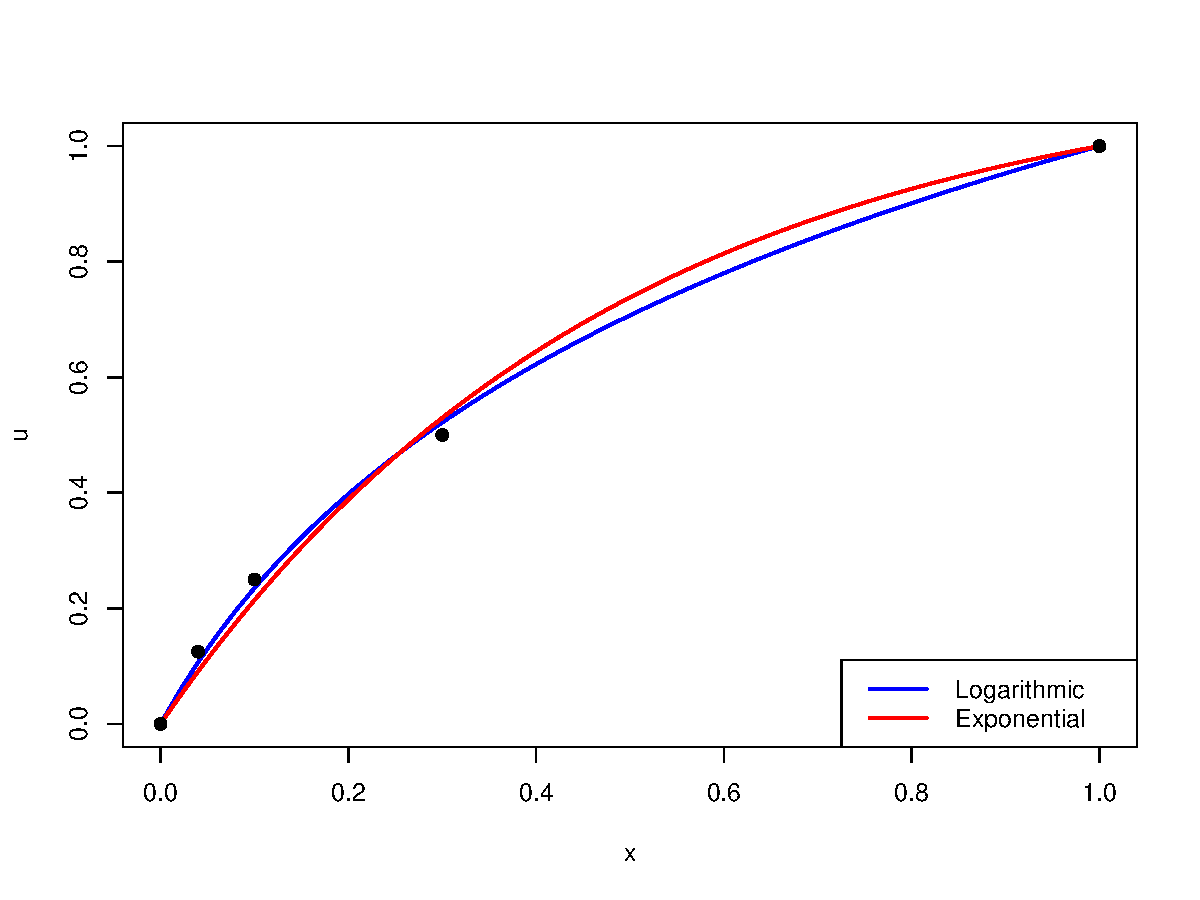
\includegraphics[width = 0.8\textwidth]{dec-fig/example-utility-fit.pdf}
	\caption{Two fitted utility functions for the example utility elicitation.}
	\label{Fig:example-elicitation}
\end{figure}

A simple least squares procedure leads to $\hat{\alpha}_{\text{exp}} = 1.143889$ and $\hat{\alpha}_{\text{log}} = 0.1795392$. Although it is apparent from \Cref{Fig:example-elicitation} that the logarithmic form provides a better fit, this can be verified numerically by considering the sum of squares; $SS_{\text{exp}} = 0.003321319 > 0.001027514 =  SS_{\text{log}}$. Prior to committing to a particular functional form we should ask at least one verification question. The elicitation did not consider $x_1$ such that $u_1(x_1) > 0.5$; we could ask a question about a value which should have a utility of at least $0.75$, say. E.g. $u_{\text{log}}(0.75 | \hat{\alpha}_{\text{log}}) = 0.873$. We could as the DM if they prefer to receive $0.8$ for sure or play the lottery $[0.3,1;0.5]$ which has expected utility $0.75$. If the fitted function is consistent with the DM's specification, they should prefer the certain option of $0.8$. Other ways to choose a utility function involve investigating the risk aversion of the DM parametrically; a constantly risk averse DM should have an exponential utility function, for example.

Now suppose we repeat the elicitation for $u_2$ and $u_3$. We obtain a set of marginal utility functions:
\begin{align}
u_1(x_1) & = 0.709+1.212\log(x+0.424) \\
u_2(x_2) & = −0.005+0.691\log(x+1.004)\\
u_3(x_3) & = 0.729+1.248\log(x+0.403).
\end{align}

One the marginal utility functions have been elicited, we need to help the DM specify the scaling constants ($k_i$) for the linear or multiplicative utility function. We will outline an example of elicitation of additive utility and multiplicative utility; for the multiplicative case we will illustrate the event that $\sum k_i > 1$ and the event that $\sum k_i < 1$. Throughout we assume $k_1>k_2>k_3$.

\subsubsection{Linear Utility}

All we have to do here is find $k_2$ and $k_3$, the linear equality constraint implies a value of $k_1$.

The DM is first asked to consider specify $\pi_2$ such that $\bx_2^* \sim [\bx_1^*, \bx^0; \pi_2]$. Suppose the DM states that $\pi_2 = 0.85$; this can be achieved asking the DM if $\bx_2^* \sim [\bx_1^*, \bx^0; \pi_2 = 0.5]$ holds and then iteratively adjusting $\pi_2$ until the DM is satisfied that the options are equally preferable. Further suppose that the DM specifies $\bx_3^* \sim [\bx_2^*, \bx^0; 0.5]$ i.e. $\pi_3 = 0.5$.

These two specifications, combined with relations $k_i = k_{i-1}\pi_i$ and \Cref{Eq:k1-soln} lead to $(k_1, k_2, k_3) = (0.46, 0.36, 0.18)$. The multiattribute utility function is then constructed by substituting each $k_i$ and $u_i$ into \Cref{Eq:add-u}.

\subsubsection{Multiplicative Utility: $\sum k_i > 1$}

Suppose as above we have $\pi_2 = 0.8$, $\pi_3 = 0.5$. We now need an extra indifference statement to obtain $k_1$. This can be obtained by asking the DM to specifty $\pi_0$ such that $\bx_1^* \sim [\bx^*, \bx^0; \pi_0]$ holds. Suppose the DM reports that $\pi_0 = 0.7$. This means that the DM thinks obtaining a good value of $x_1$ is very important. From this it is easy to see $k_1 = \pi_0$ since $U(\bx^*_1) = \E \{ [\bx^*, \bx^0; \pi_0] \} = \pi_0.$ Then using $k_i = k_{i-1} \pi_i$ we obtain $(k_1, k_2, k_3) = (0.7, 0.56, 0.28)$ with $\sum k_i = 1.54$. To finalise the utility function we need to obtain $k$; we just employ \Cref{Eq:k-soln} which in this case leads to a quadratic in $k$ (we can divide through by $k$ since $k = 0$ is not a valid solution). However there is only one permissible solution, for utility independence properties of \Cref{Eq:mult-u} to hold it must be the case that $k \in (-1, 0)$. Therefore the in this case $k = -0.83$ (the other solution to the quadratic is $k \approx -6$). Then $u(\bx)$ is constructed by substituing the $k_i$, $k$ and the $u_i$ into \Cref{Eq:mult-u}.

\subsubsection{Multiplicative Utility: $\sum k_i < 1$}

The procedure for $\sum k_i < 1$ is essentially the same as for when $\sum k_i > 1$ except for the DM's utility independence properties to hold, we must have $k>0$.

Now to elicit $k_1$ we again consider two equally preferable options: $\bx_1^* \sim [\bx^*, \bx^0; \pi_0]$. Suppose, in this scenario that $\pi_0 = 0.3$. This then leads to $(k_1, k_2, k_3) = (0.3, 0.24, 0.12)$, hence $\sum k_i = 0.66<1$. We then have to solve \Cref{Eq:k-soln} subject to $k>0$. This leads to $k = 0.218$ (the other solution to the quadratic is $k \approx -18$).

\section{Biases}

DM's exhibit two main forms of bias: cognitive (e.g. overconfidence) or motivational (e.g. wishful thinking). Further, group based decision making also has biases. We will review these forms of biases and discuss how to combat them. This chapter is based on \citet{Montibeller2018}.

\subsection{Relevant Individual Biases}

A cognitive bias is a systematic difference between the ``true'' answer and an elicited value. The term ``debias'' refers to methods to eliminate, but more realistically reduce, the cognitive or motivational bias.

\subsubsection{Relevant Individual Cognitive Biases}

\textbf{Anchoring.}
When estimating a quantity, an anchor (initial value) might be provided to the DM. The idea is to adjust this value to a ``final'' answer, the DM is likely to not sufficient adjust the anchor value enough. To debias: avoid anchors; provide multiple or counter-anchors; use multiple experts.

\noindent\textbf{Availability.}
The elicited probability of an event depends on how easy it is recalled --- not how likely the event is. To debias: provide probability training; give counter examples; provide data.

\noindent\textbf{Certainty Effect.}
DMs prefer certainties over gambles with similar expected utility. Occurs in elictations employing probability vs certainty equivalents: these methods produce different results. To debias: avoid certainties; separate value and utility elicitation; explore relative risk parametrically.

\noindent\textbf{Equalising.} DMs allocate similar weight/probability to all objectives/events. To debias: rank objectives prior to weighting; elicit weights or probabilities hierarchically.

\noindent\textbf{Gain-Loss.} Alternate farmings of a problem (as a loss or gain) may lead to different answers. To debias: clearly identify the status quo (SQ); for value functions, express values as marginal changes from SQ; elicit gains and losses separately for utility functions; cross check utility for mixed gambles to verify consistency.

\noindent\textbf{Myopic Problem Representation.} The problem at hand is oversimplified leading to a reduced number of objectives or future states of the world. To debias: encourage DMs to think of more objectives/alternatives/possible future states; involve multiple experts/stakeholders improving the range of objectives/alternatives/future states.

\noindent\textbf{Omission of Important Variables.} One (or more) important variables is not included in the problem, possibly overlooked. To debias: prompt for alternatives and objectives; ask for extreme or unusual situations; use group elicitations.

\noindent\textbf{Overconfidence.} Estimates of parameters indicate overperformance (overestimation) or interval estimates are too narrow (over-precision). To debias: initialise elictations at extreme values; avoid central tendency anchors; use fixed value rather than fixed probability elicitation.

\noindent\textbf{Splitting Biases.} The grouping of objectives affects their elicited weights. Alternatively, the way events are grouped in a fault tree affects their probabilities. To debias: split objectives/events with high weight/probability; don't split objectives/events with low probability; use hierarchical estimation techniques; use ratio judgements instead of direct estimation.

\noindent\textbf{Proxy Bias.} Proxy attributes receive more weight than their respective fundamental objective. To debias: avoid proxies; build models relating the proxy to fundamental objectives; provide weights for fundamental objectives.

\noindent\textbf{Range Insensitivity.} The weights of objectives are not properly adjusted to changes in the range of an attribute. To debias: make ranges explicit; use swing weighting; use trade-off or pricing out procedures.

\noindent\textbf{Scaling.} This is a group of stimulus-response biases: \textit{contraction bias}, \textit{logarithmic response bias}, \textit{range equalising bias}, \textit{centering bias}, \textit{equal frequency bias}. To debias: develop scales which match stimuli response; choose appropriate scaling techniques for the required measurement.

\subsubsection{Motivational Biases}

Motivational biases are those in which judgements are impacted by how preferable an event, choice or consequence is. Experts might provide optimistic forecasts for desirable outcomes. Motivational bias might be the \textit{deliberate} attempt to provide optimistic forecasts. However they not be conscious; for example the estimated time to complete a software project is frequently underestimated.

\noindent\textbf{Affect-Influence.} The preference for (or against) a particular outcome taints the judgement. To debias: cross-check elicitations; use multiple experts (with differing points of view); multiple elicitation protocols.

\noindent\textbf{Confirmation.} This is the bias in which one confirms existing beliefs, this leads to selectivity in the use and gain of evidence. To debias: use multiple experts; provide counterfactuals; probe for evidence.

\noindent\textbf{Desirability of Positives.} The stated probability of an outcome depends on how desirable it is deemed by the DM. Same as ``wishful thinking''. To debias: use multiple experts; use scoring rules.

\noindent\textbf{Undesirability of Negatives.} The DM's aversion to negative consequences causes them to give conservative estimates of harmful consequences. To debias: use multiple experts; use scoring rules.


In summary, there are many biases the elicitation must overcome. The most frequently required debiasing techniques are: using multiple experts, prompting DMs/experts about scenarios and objectives, providing counter examples, cross-checking elicitations and avoiding anchors. It seems to be the case that motivational biases primarily affect the elictation of probability whereas cognitive biases have an impact on the elicitation of both probability and utility.
\section{Sensitivity Analysis for Decision Theory}

Frequently, a complex computer model may be used in the decision analysis. Denote the computer model as $\eta(\cdot)$ with (uncertain) inputs $\bX$ It is common in computer modelling to conduct a ``global'' sensitivity analysis (SA). Variance based SA \citep{Sobol1993,Oakley04} is used to understand the relative importance of subgroups of $\bX$. Note that a ``subgroup'' of $\bX$ might be, and often is, just an individual component of $\bX$.

The variance based sensitivity analysis is of interest to the model user, but does not take into account the \textit{purpose} of the model. The model has likely been designed to aid a decision making process. Hence the sensitivity analysis should assess how input uncertainty impacts the DM's final (optimal) decision and their utility/loss function.

Suppose the decision maker must choose a decision $d \in \mathcal{D}$ where $\mathcal{D}$ is the space of all possible decisions. The DM's utility for decision $d$ will depend on the simulator output $Y = \eta(\bX)$ where $\bX = \{X_1, \ldots, X_r \}$ are the ``true'' values of the unknown inputs. If we write the DM's utility function as $U\{ d, \eta(\bX) \}$ then the expected utility of this decision (given no new information) is

\begin{equation}
U^*  = \max_{d \in \mathcal{D}} \E_{\bX} \left[ U \{ d, \eta(\bX) \} \right].
\end{equation}

Now suppose the DM wants to consider how $X_i$ impacts their expected utility. Assuming each $X_i$ is equally difficult to obtain, the expected value of learning $X_i$ prior to making the decision is

\begin{equation}
E_{X_i} \left[ \max_{d \in \mathcal{D}} \E_{\bX | X_i} \left[ U \{ d, \eta(\bX) \} \right] \right] - U^*. \label{Eq:p-evpi}
\end{equation}

In health economics, \Cref{Eq:p-evpi} is referred to at the \textit{partial expected value of perfect information} (partial EVPI) for input $X_i$. This quantity relates the importance of uncertainty in $X_i$ to the decision problem.

\subsection{Variance Based Sensitivity Analysis is a Special Case of EVPI}

If $Y$ is scalar then the importance of $X_i$ is given by

\begin{equation}
	\var_{X_i} \left\{ \E( Y|X_i) \right\} \label{Eq:vbsa}
\end{equation}

usually this is normalised by $\var(Y)$ so that the importances are on $[0,1]$. Now since
\begin{equation}
\var_{X_i} \left\{ \E( Y|X_i) \right\} = \var(Y) - \E_{X_i} \left\{ \var(Y|X_i) \right\}.
\end{equation}

If the decision problem is the estimation of $Y$ and the DM chooses the utility function $U(d, \eta(\bX)) = -(d - \eta(\bX))^2$ (quadratic loss of estimation error) as their utility function then the measurement given by \Cref{Eq:vbsa} is equivalent to partial EVPI under the quadratic loss utility function. Proof given in \Cref{sec:evpi-proof}.
These variance based measures are not completely redundant; they form part of an exploratory analysis. If the quadratic loss function is not the appropriate utility function, variance based sensitivity analysis does not quantify the input importance in the correct way.

Consider an example in which the DM is concerned as to whether $Y$ is above some critical threshold. Let $\mathcal{D} = \{ d_1, d_2 \}$ and $d_1 \succ d_2$ if $Y>0$. Now consider the following density plot

\begin{figure}
	\centering
	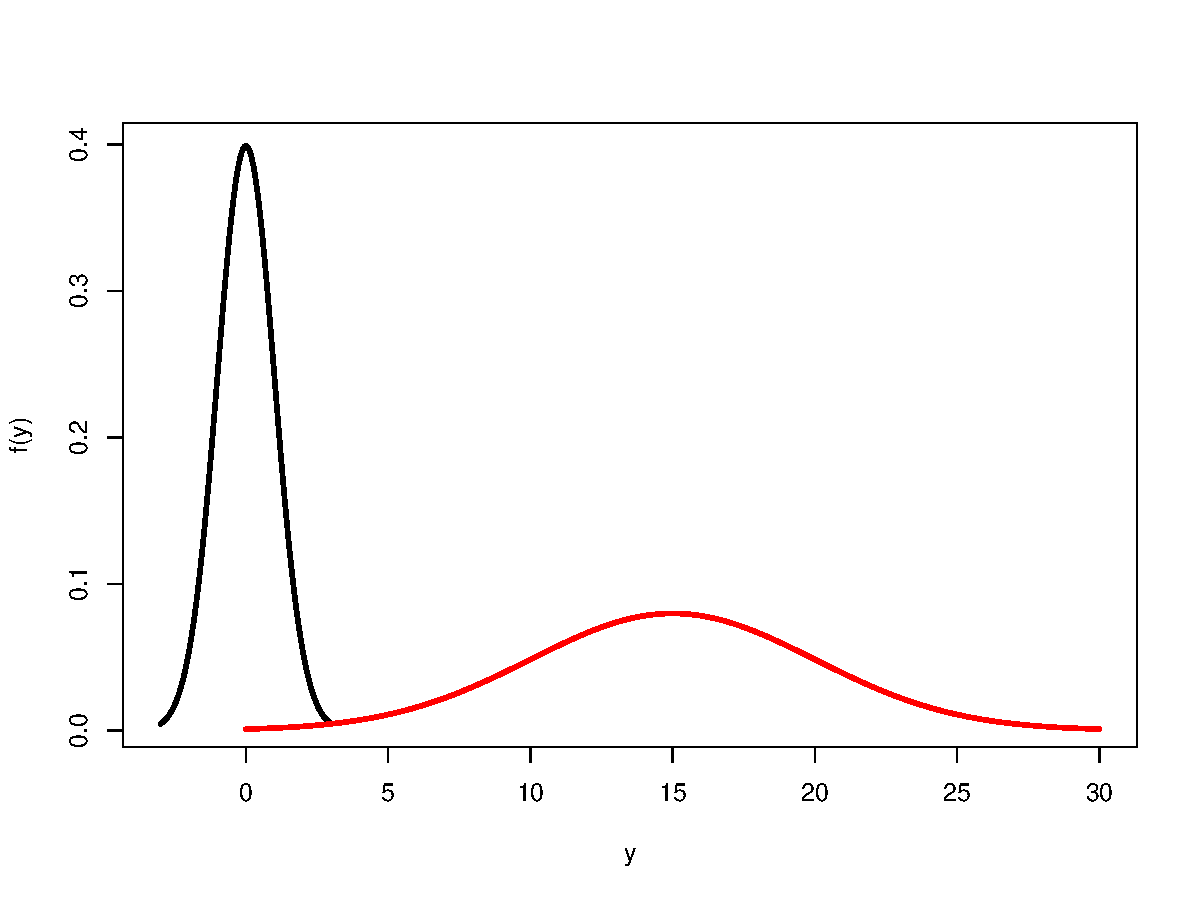
\includegraphics[width = 0.7\textwidth]{dec-fig/y-density.pdf}
	\caption{Two possible probability densities for $Y$.}
	\label{Fig:y-density}
\end{figure}

Clearly in \Cref{Fig:y-density} the red density has greatest uncertainty about $Y$. However, the red density satisfies $Y>0$ with \textit{no uncertainty}. Uncertainty about the \textit{best decision} is greatest in the black density.

\subsection{Computation of Partial EVPI with GPs}

The simplest approach is to simply replace $\eta(\bx)$ with a fast surrogate; the GP posterior mean $m^{\star}(\bx)$. We can then proceed via a Monte Carlo approach.

However, we consider a particular class of decision problem where $\mathcal{D} = \{1, \ldots, s\}$ where $s$ is quite small. Now to link the simulator output to the DM's utility, we assume that $\eta(\bx)$ returns the vector output $\{\eta_1(\bx), \ldots, \eta_s(\bx) \}$, with

\begin{equation}
	\eta_d(\bx) = U\{ d , \eta(\bx) \}
\end{equation}

this seems to be a more sensible approach when $\eta(\cdot)$ is deterministic. If $\eta(\cdot)$ is stochastic, a Monte Carlo approach may be more straightforward.

for each $d \in \mathcal{D}$. Each $\eta_d(\bX)$ is the ``true'', utility of decision $d$. We construct a separate GP emulator for each $\eta_d(\bx)$ with data $\by_d$ and GP parameters $\Theta_d$.

We treat each $\eta_d$ as an unknown; as are each $\bX$. Therefore, to find the expected utility of a decision, this expectation needs be be taken with respect to $\bX$ \textit{and} $\eta_d$. Therefore
\begin{equation}
\E_{\eta_d} \left[  \E_{\bX}\left[ U\{ d, \eta(\bX) \} \right] | \by_d, \Theta_d \right]
=
\E_{\eta_d} \left[  \E_{\bX}\left[ \eta_d(\bX) \right] | \by_d, \Theta_d \right].
\end{equation}

Hence, when $\eta_d$ is unknown, the partial EPVI of $X_i$ is

\begin{equation}
v_i = \E_{X_i} \left[ \max_{d \in \mathcal{D} } E_{\eta_d} \left\{ \E_{\bX|X_i} \left\{ \eta_d(\bX) \right\}  | \by_d, \Theta_d \right\} \right] - \max_{d \in \mathcal{D}} \E_{\eta_d} \left[ \E_{\bX} \left\{ \eta_d (\bX) \right\} | \by_d, \Theta_d \right].
\end{equation}

\subsection{Uncertainty Quantification}

Partial EVPI will depend on the DM's current beliefs about $\eta_d(\cdot)$ and also, the constructed emulators are conditional on the diagonal matrix of correlation lengthscales, $B_d$. To quantify uncertainty in $v_i$ we require $p(v_i | \by_d)$. In writing $\mathcal{B} = \{B_1,\ldots,B_n\}$, approximate draws from $p(v_i | \by_d)$ are available by sampling from

\begin{equation*}
p(v_i, \mathcal{B}, \eta(\cdot)| \by) = p(\mathcal{B}|\by)p(\eta(\cdot)|\mathcal{B}, \by)p(v_i | \mathcal{B}, \eta(\cdot), \by)
\end{equation*}
where $v_i$ is deterministic conditional on $\eta(\cdot)$. MCMC allows for sampling from $p( \mathcal{B}| \by )$ Sampling from the other distributions is more complex and is discussed by \citet{Oakley2009}.
%%%%%%%%%%%%%%%%%%%%%%%%%%%%%%%%%%%%%%%
%%%%%%%%%%%%%%%%%%%%%%%%%%%%%%%%%%%%%%%
%%%%%%%%%%%%%%%%%%%%%%%%%%%%%%%%%%%%%%%
%%	      APPENDIX		     %%
%%%%%%%%%%%%%%%%%%%%%%%%%%%%%%%%%%%%%%%
%%%%%%%%%%%%%%%%%%%%%%%%%%%%%%%%%%%%%%%
%%%%%%%%%%%%%%%%%%%%%%%%%%%%%%%%%%%%%%%



\subsection*{EVPI Proof \label{sec:evpi-proof}}

Here we present the proof that partial EVPI is equivalent to variance based sensitivity analysis under quadratic loss. To frame this as a decision problem, we consider the ``decision'' of estimating the output of a complex computer model; the estimation is via a GP emulator and our utility function is $U(d) = -(d - \eta(\bX))^2$.

The partial EVPI of $\bX_i$ is
\begin{align}
&\E_{\bX_i} \left\{ \max_{d} \E_{\bX_{-i|i}} \left[ U(d, \eta(\bX) \right] \right\} - \max_d \E_{\bX} \left[ U(d, \eta(\bX) \right]& \\
&=\E_{\bX_i} \left\{ \max_{d} \E_{\bX_{-i|i}} \left[ -(d - \eta(\bX))^2 \right] \right\} - \max_d \E_{\bX} \left[ -(d - \eta(\bX))^2) \right]\\
& = \E_{\bX_i} \left\{ \max_{d}  \left[ -d^2 + 2d \E_{\bX_{-i|i}}(Y) - \E_{\bX_{-i|i}}(Y)^2 \right] \right\} - \max_d \left[-d^2 + 2d \E_{\bX} (Y) - \E_{\bX} (Y)^2 \right]
\end{align}

where $Y = \eta(\bX)$.

We now need to perform the maximisations. To do this, we will define a new function

\begin{equation}
\theta(t) = -t^2 + 2at - a^2
\end{equation}

which has obvious similarities with the above functions to be maximised.

Differentiating $\theta$ with respect to $t$ and equating to $0$ gives


\begin{equation}
\frac{\dd \theta}{\dd t} = -2t + 2a   = 0\\.
\end{equation}

Clearly $t = a$ solves this equation and it is straightforward to show that this is indeed the global maximum.

Now setting $t = d$ and $a = \E_{\bx_{-i|i}}(Y)$ shows the first maximisation is satisfied at $d = \E_{\bX_{-i|i}} (Y)$. Similarly, the second maximisation is achieved at $d = \E_{\bX} (Y)$.

Now the partial EVPI can be expressed as

\begin{align}
&\E_{\bX_i} \left\{ \E_{\bX_{-i|i}}(Y)^2 - \E_{\bX_{-i|i}}(Y^2) \right\} - \left(\E_{\bX}(Y)^2 - \E_{\bX}(Y^2)\right)\\
&= \var_{\bX}(Y) - \E_{\bX_i} \left\{ \var_{\bX_{-i|i}}(Y) \right\}
\end{align}
which completes the proof. Note that EVPIs are unnormalised whereas in variance based sensitivity analysis it is common to normalise by $\var(Y)$. 
%% references
\end{chapter}
